This chapter presents our approach to Vision-and-Language Navigation (VLN) for autonomous driving in dynamic outdoor environments.\footnote{This chapter is based on Jain et al., \textit{Ground then Navigate: Language-guided Navigation in Dynamic Scenes}, IEEE ICRA 2023~\cite{jain2023ground}.} Building on the CARLA-NAV dataset introduced in Chapter~\ref{ch:dataset}, we formalize the problem, describe a multi-task grounding network, explain live navigation, and report quantitative and qualitative results. Dataset creation details are not repeated here; we focus on modeling, inference, and evaluation.

\section{Background and Related Work}

Chapter~\ref{ch:background} already taxonomizes VLN families and maps gaps A--C; here we only add method-level citations for visual grounding that feed our formulation. Visual grounding associates linguistic descriptions with visual counterparts via proposal-based Referring Expression Comprehension (REC)~\cite{rohrbach2016grounding,hu2016natural,plummer2018conditional,rufus2020cosine,deng2018visual,zhang2018grounding,yang2019dynamic,qiu2020language} or pixel-level Referring Image Segmentation (RIS)~\cite{shi2018key,ye2019cross,huang2020referring,jain2021comprehensive}. Referring Navigable Regions (RNR)~\cite{Rufus_2021} localizes navigable road regions for language commands, but is limited to static images in pre-recorded sequences~\cite{caesar2020nuscenes}. We reformulate RNR for dynamic outdoor settings and perform live navigation with continuous control via a local planner. Continuous-control grounding of free-form navigable regions remains comparatively rare relative to discrete-action outdoor VLN.

\section{Problem Statement}

Having situated the task against prior work, we now state the prediction problem the network must solve. Intuitively, the network continuously predicts the next drivable region rather than the final destination: the command says which region, and the past trajectory says how much of the command is already done.

Given video frames $V=\{v_{t-k}, v_{t-k+1}, \ldots, v_{t}\}$, a contextual historical trajectory $P$, and a language command $L = \{l_1, l_2, \ldots, l_N\}$, where $t$ is the current timestamp, $k$ is the historical window size, and $N$ is the maximum number of words, the goal is to predict the navigable mask $y_t$ and the future trajectory mask $z_t$ for the current frame $v_t$.

The contextual trajectory $P$ provides information about which part of a multi-step command has already been executed. For example, for ``turn left and park near the blue dustbin,'' $P$ indicates whether the left turn has already been taken. The spatial location of the navigation mask should determine the trajectory path's direction, and vice versa.

\section{Formal Analysis}
\label{sec:formal_analysis}

Before describing the architecture, we state why a dense grounding-first formulation is a better inductive bias for outdoor language-guided driving than selecting from a small discrete action set.

\subsection{Why Segmentation Dominates Discrete Action Selection}

Intuitively, with a fixed menu of four actions there are places on the road the vehicle simply cannot be asked to go, no matter how much data it sees. Let $\mathcal{A}_{\mathrm{disc}}=\{a_1,\ldots,a_K\}$ be a finite action alphabet (e.g., FORWARD, LEFT, RIGHT, STOP as in Touchdown-style outdoor VLN~\cite{Chen2019TOUCHDOWN}). Executing a sequence drawn from $\mathcal{A}_{\mathrm{disc}}$ induces a finite reachable set $\mathcal{R}_{\mathrm{disc}}$ of vehicle poses relative to the current state. The set of drivable poses on the road, $\mathcal{R}_{\mathrm{road}}$, is a continuum: any point on the free surface is in principle a legal target. The Hausdorff gap
\begin{equation}
    \delta = \sup_{x \in \mathcal{R}_{\mathrm{road}}} \inf_{y \in \mathcal{R}_{\mathrm{disc}}} \|x-y\|
\end{equation}
is an irreducible quantization error of discrete control. Commands such as ``park between the two cars on the right'' require placing the vehicle at a geometrically constrained pose that typically lies outside $\mathcal{R}_{\mathrm{disc}}$ for small $K$. The failure is therefore \emph{representational}, not statistical: no amount of additional discrete-action data recovers a maneuver that the action space cannot express. By contrast, predicting a navigable-region mask $y_t$ and taking its centroid (or any point sampled from the mask) as a planner target yields a goal in continuous world coordinates, so the reachable set under a competent local planner approximates $\mathcal{R}_{\mathrm{road}}$ up to planner fidelity rather than up to $K$.

\subsection{Advantages of Grounding-First}

Intuitively, the network decides \emph{where} to go; the planner decides \emph{how}. We factorize the policy as
\begin{equation}
    P(\mathrm{controls}\mid V,P,L) \;=\; P_{\mathrm{plan}}(\mathrm{controls}\mid y_t,\;\mathrm{state})\; P_\theta(y_t\mid V,P,L),
\end{equation}
where $P_\theta$ is the learned grounding network and $P_{\mathrm{plan}}$ is a fixed local planner. Three consequences follow:

\begin{enumerate}
    \item \textbf{Supervision density.} Each frame provides $O(HW)$ pixel-level targets for $y_t$, versus a single categorical label under action classification. Dense losses (Eq.~\ref{eq:combo_loss}) therefore supply far richer gradient signal per demonstration.
    \item \textbf{Dynamics as a prior.} Vehicle kinematics and collision avoidance enter through $P_{\mathrm{plan}}$ rather than being relearned inside $P_\theta$.
    \item \textbf{Inspectability.} Every decision yields an explicit mask that can be visualized and overridden. This is the operational basis of the interpretability claim, not a post-hoc explanation of a black-box action logit.
\end{enumerate}

The short-term trajectory head $z_t$ is an auxiliary dense prediction that shares $M$ with the navigation head; it does not enter $P_{\mathrm{plan}}$ in the current system, but correlates with $y_t$ and provides a visual cue of the intended short-horizon path. Early project drafts independently noted that incorporating the predicted trajectory into the planner is future work, confirming that the published system uses $z_t$ for interpretability rather than control.

\subsection{Complexity of Multimodal Fusion}

Multi-head self-attention in Eq.~\ref{eq:vln_attention} operates over $S=(T{+}1)+N$ multimodal tokens at spatial resolution $HW$. With $T=8$, $H=W=7$, and $N\le 20$, we have $HW=49$ spatial sites and on the order of $S\cdot HW \approx 441$ tokens when language is broadcast spatially (or $S$ tokens after spatial pooling, depending on implementation). Self-attention is quadratic in the attended length, so the dominant cost scales as $O\bigl(((T{+}1)\,HW)^2 C\bigr)$ when attending over the visual--trajectory grid. Doubling the frame count therefore roughly quadruples attention FLOPs. This motivates stopping the frame ablation at $n=8$ (Table~\ref{table:frame_ablation}) and predicting only every fifth frame at inference time. Trainable parameters are concentrated in the fusion block and two segmentation heads; the CLIP ViT-B/32 encoders contribute the majority of total parameters.

\subsection{Convergence Intuition for Combo Loss}
\label{sec:combo_intuition}

Navigable masks cover a small fraction of each frame, so the pixel prior is heavily skewed toward background. The BCE term $L_{\mathrm{bce}}$ then yields gradients dominated by easy negatives. The soft Dice coefficient $D(\hat{y}_t,y_t)$ is (approximately) scale-invariant to foreground size and directly optimizes overlap, counteracting that skew. Setting $\lambda=0.3$ weights the objective toward Dice while retaining a calibrated probabilistic BCE term for stable early training~\cite{taghanaki2019combo}. Both heads share the same $L_{\mathrm{combo}}$; balancing them amounts to summing the two losses with equal weight in our experiments. Severe class imbalance and the small absolute mask area also explain why area-based stopping is sensitive: area growth under perspective is a coarse proxy for goal proximity.

\section{Methodology}
\label{sec:methodology}

The formal analysis above motivates a dense, multi-task architecture; we now specify its components. We propose a multi-task network for navigation-region prediction and future-trajectory prediction (Contribution~\ref{contrib:network}). Both tasks are treated as dense prediction tasks for interpretability. During live inference, dense pixel points are converted to 3D world coordinates using inverse projective transformation. As shown in Figure~\ref{fig:proposed_pipeline}, every output is a mask before the planner is invoked.

\begin{figure*}[ht]
\centering
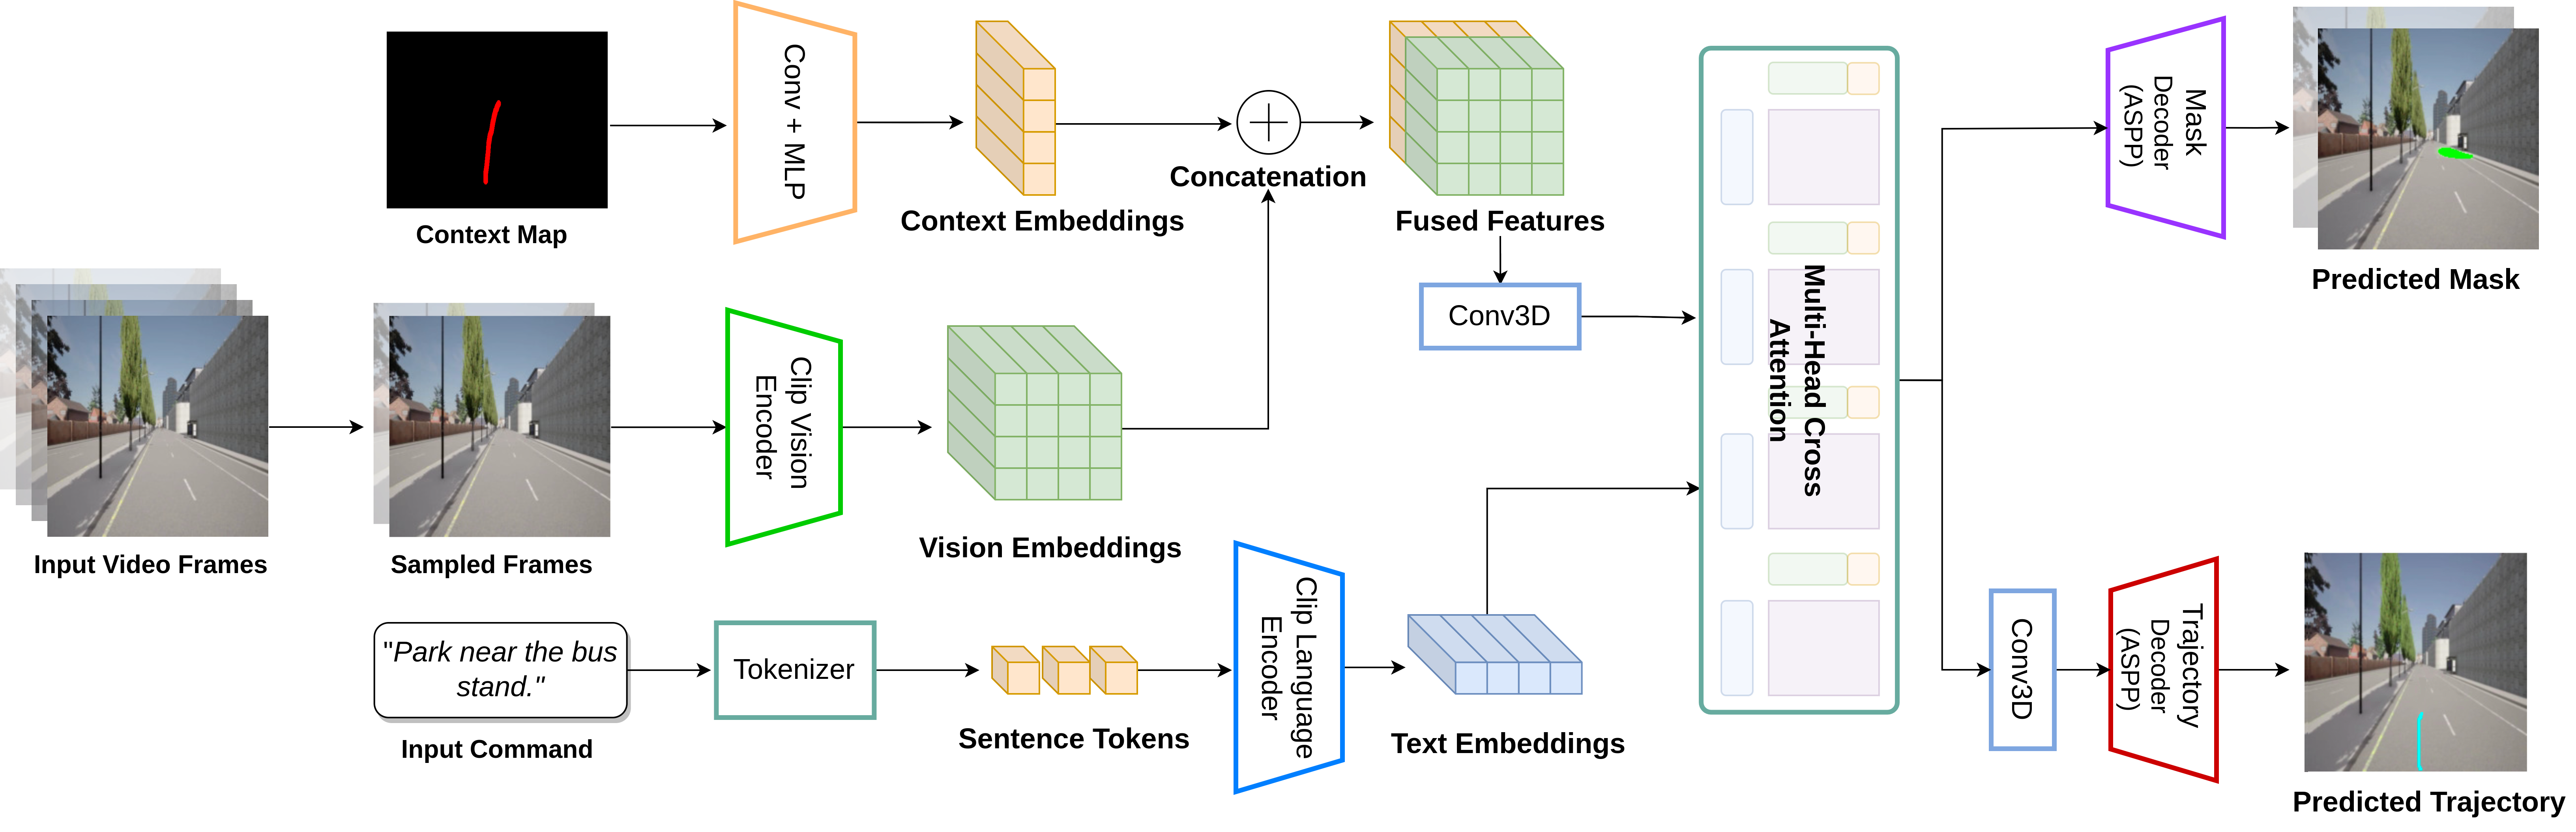
\includegraphics[width=0.98\textwidth]{figures/vln/method_pipeline_figure.png}
\caption[Proposed multi-task grounding pipeline]{Overall pipeline of the proposed approach (Contribution~\ref{contrib:network}). Given visual frames, the already executed past trajectory, and the textual command, the network predicts a navigable-region mask and a short-horizon trajectory mask. Every output is a mask, so every decision is inspectable before it reaches the planner.}
\label{fig:proposed_pipeline}
\end{figure*}

\subsection{Feature Extraction}

We utilize CLIP~\cite{radford2021learning} to extract linguistic and visual features. For the linguistic expression $L$, we tokenize the command with the CLIP tokenizer and obtain word-level features $F^l = \{f^{l}_{1}, \ldots, f^{l}_{N}\}$ of shape $\mathbb{R}^{N \times C_l}$. For visual frames $V$, CLIP encodes video features $F^v=\{f^{v}_{t-k}, \ldots, f^{v}_{t}\}$. For trajectory context $P$, we project the past trajectory onto an image of the same size as $v_t$ and pass it through convolution and MLP layers to obtain $F^p$ with the same feature size as the per-frame visual features.

\subsection{Multi-Modal Fusion}

Intuitively, we lay the frames, the past-trajectory image, and the words out as one sequence and let attention decide which words attend to which places and times. The trajectory context feature $F^p \in \mathbb{R}^{C_v \times 1 \times HW}$ is concatenated with video features $F^v$ along the temporal dimension, yielding $F^{vp} \in \mathbb{R}^{C_v \times (T+1) \times HW}$. We then fuse $F^{vp}$ with linguistic features $F^l \in \mathbb{R}^{N \times C_l}$ by length-wise concatenation along the sequence axis (denoted $[\cdot;\cdot]$ to avoid confusion with the Hadamard product), apply multi-head self-attention over the resulting multimodal tokens, and collapse the temporal axis with a 3D convolution:
\begin{equation} \label{eq:vln_attention}
\begin{split}
    F &= [F^{vp}; F^l] \in \mathbb{R}^{C \times S \times HW}, \\
    A &= \mathrm{Mhead}(F, F, F), \\
    M &= \mathrm{Conv3D}(A F) \in \mathbb{R}^{C_m \times H \times W},
\end{split}
\end{equation}
where $S = (T{+}1) + N$ is the joint token length after concatenation, $\mathrm{Mhead}$ is multi-head self-attention over the multimodal sequence, $A F$ denotes matrix multiplication of the attention weights with the value features, and $\mathrm{Conv3D}$ aggregates the temporal (and language) axis into a single spatial feature map $M$ for the segmentation heads.

\subsection{Segmentation Heads and Loss}

Separate segmentation heads (sequences of convolutions with upsampling) predict the navigation and trajectory masks from $M$. We train with combo loss~\cite{taghanaki2019combo}, a combination of pixel-wise binary cross-entropy and the Dice coefficient used as a soft overlap term. Intuitively, the mask is a small target in a big image, so a per-pixel loss can score well by predicting ``not navigable'' everywhere; Dice measures overlap and cannot be gamed that way (Section~\ref{sec:combo_intuition}):
\begin{equation} \label{eq:combo_loss}
\begin{split}
    L_{\mathrm{bce}} &= -\frac{1}{|\Omega|}\sum_{i \in \Omega}\bigl(y_{t,i}\log(\hat{y}_{t,i}) + (1 - y_{t,i})\log(1 - \hat{y}_{t,i})\bigr),\\
    D(\hat{y}_{t}, y_{t}) &= \frac{2\sum_{i}\hat{y}_{t,i}\, y_{t,i}}{\sum_{i}\hat{y}_{t,i} + \sum_{i} y_{t,i} + \varepsilon},\\
    L_{\mathrm{combo}} &= \lambda L_{\mathrm{bce}} - (1 - \lambda)\, D(\hat{y}_{t}, y_{t}),
\end{split}
\end{equation}
where $\Omega$ indexes image pixels and $\varepsilon$ is a small constant for numerical stability. We set $\lambda = 0.3$ so that the Dice term dominates. The same loss is applied to both heads; the approach is end-to-end trainable, and the predicted trajectory correlates with the predicted navigation mask as a short-term route cue.

\subsection{Live Navigation}
\label{sec:live_nav}

To convert predictions into closed-loop driving, we next specify how masks become planner targets (Contribution~\ref{contrib:live}). We take the largest connected component and use its centroid as the 3D goal (via inverse projective transform). As the vehicle approaches the final region, the predicted mask area tends to increase due to perspective; we therefore use an area-based rule to decide when to stop. Algorithm~\ref{alg:target} summarizes the decision procedure used in the published CLIP-family experiments.

\begin{algorithm}[ht]
\caption{Target determination for live navigation (CLIP-family protocol)}
\label{alg:target}
\begin{algorithmic}[1]
\Require Predicted navigable mask $\mathbf{M}$, trajectory mask $\mathbf{T}$ (optional)
\State Threshold $\mathbf{M}$ and extract connected components
\State Let $C$ be the component with largest summed probability; $c \leftarrow$ weighted centroid of $C$
\If{area of $C$ exceeds an empirically chosen threshold for five consecutive predictions}
    \State Treat $c$ as the final goal and stop navigation
\Else
    \State Pass $c$ to the local planner as the next intermediate target
\EndIf
\end{algorithmic}
\end{algorithm}

The numeric area threshold was found empirically and was \emph{not} recorded in the archival paper or earlier drafts; we therefore do not invent a value here. During inference we predict every 5 frames to reduce latency; training uses every frame of each episode.

\paragraph{Evolution of the stopping rule.}
The live-navigation rule evolved across project drafts, and documenting that evolution clarifies what the CLIP tables actually measure:
\begin{enumerate}
    \item \textbf{Two-class mask with trajectory fallback.} Early prototypes predicted separate intermediate and final mask channels. The target was the weighted centroid of the dominant component; if neither channel exceeded a confidence threshold $\delta$, the farthest point of the skeletonized trajectory mask was used instead. Three consecutive final predictions ended the episode.
    \item \textbf{Two-band confidence counters.} An intermediate draft averaged the intermediate and final channels, applied $\delta_{\min}$/$\delta_{\max}$ bands, incremented a confident-prediction counter, and ended after a short no-new-target timeout.
    \item \textbf{Single-mask area rule (reported).} The ICRA protocol, and all CLIP results in this chapter, uses a single navigable mask with five consecutive area triggers (Algorithm~\ref{alg:target}).
\end{enumerate}

\section{Evaluation Metrics}
\label{sec:eval_metrics}

With the live pipeline defined, we next choose metrics that match the set-valued nature of language commands. Following prior VLN work~\cite{schumann-riezler-2022-analyzing,xiang-etal-2020-learning,Chen2019TOUCHDOWN}, we use \textbf{Task Completion (TC)} as the primary success metric: whether the agent successfully navigates to the goal location for a given language command. Importantly, TC in our evaluation is a \emph{human} judgment of episode success rather than an automatic geometric check; inter-rater agreement was not recorded. We additionally use \textbf{Fr\'{e}chet Distance}~\cite{eiter1994computing} and \textbf{normalized Dynamic Time Warping (nDTW)}~\cite{ilharco2019general} to compare the live predicted path with the ground-truth path.

Fr\'{e}chet Distance and nDTW provide useful path-similarity signals, but they are not fully robust indicators of average navigation quality: a single early wrong turn can dominate the score, and a linguistic command may admit multiple valid trajectories (e.g., ``park near the blue dustbin''). Task Completion therefore remains the primary metric, with the caveat that it inherits subjectivity from human labeling. Section~\ref{sec:metric_validity} develops this construct-validity argument in full and motivates a reproducible goal-region success predicate (Section~\ref{sec:reproducible_tc}).

Because live CARLA evaluation is stochastic under dynamic traffic, we also report Wilson score 95\% confidence intervals for TC (Table~\ref{table:tc_ci}), computed from the binomial success counts implied by the point estimates on $n_{\mathrm{val}}=25$ and $n_{\mathrm{test}}=34$ episodes. These intervals quantify sampling uncertainty of a single evaluation pass under a binomial model; they do \emph{not} capture annotator disagreement, and they are not a substitute for multi-seed re-runs (Section~\ref{sec:extended_eval}).

\subsection{Displacement Metrics for Preliminary Models}
\label{sec:disp_metrics}

Before adopting CLIP and Task Completion, earlier model variants were evaluated with trajectory-displacement metrics that remain useful for stratified analysis. Let $A=(a_1,\ldots,a_{T_A})$ and $B=(b_1,\ldots,b_{T_B})$ be predicted and ground-truth trajectories in world coordinates (CARLA meters).

\begin{itemize}
    \item \textbf{Final Displacement Error (FDE):} $L_2$ distance between the terminal points, $\|a_{T_A}-b_{T_B}\|_2$.
    \item \textbf{Average Displacement Error (ADE):} mean $L_2$ distance after resampling both paths to a common length $T$, $\frac{1}{T}\sum_{i=1}^{T}\|a_i-b_i\|_2$.
    \item \textbf{ADE-Match:} because ADE requires equal-length trajectories, the preliminary evaluation used a coupling-based variant that replaces the Fr\'{e}chet supremum with a mean over the coupling. Intuitively, this metric can be fooled: an agent that stalls in one place can score near zero. With continuous reparameterizations $\alpha,\beta:[0,1]\to[0,1]$,
    \[
    \mathrm{ADE{-}Match}(A,B)=\inf_{\alpha,\beta}\;\underset{t\in[0,1]}{\mathrm{mean}}\; d\bigl(A(\alpha(t)),B(\beta(t))\bigr).
    \]
    This quantity is closely related to the \emph{average} (integral) Fr\'{e}chet Distance introduced by Buchin~\cite{buchin2007frechet} and studied algorithmically by Maheshwari et al.~\cite{maheshwari2015integral}: the standard formulation integrates distances with respect to \emph{arc length} and normalizes by curve length. The uniform-in-$t$ infimum above is degenerate: a monotone reparameterization can linger near one point of $B$ for almost the whole interval and sweep the remainder over vanishing measure, so a stalled agent can approach zero. We report ADE-Match as computed in the preliminary ViT/Conv3D evaluation (Section~\ref{sec:prelim_arch}) and interpret it with that caveat.
\end{itemize}

\subsection{Construct Validity: Why Task Completion Is Primary}
\label{sec:metric_validity}

Intuitively, ``park near the blue dustbin'' does not name one path; it names a family of acceptable ones, and a metric that compares against one recorded path will punish the acceptable alternatives. A language command $C$ does not designate a single trajectory. It designates a \emph{set} $\Phi(C)$ of trajectories that satisfy the command. The recorded demonstration $\tau^\star$ is one sample from $\Phi(C)$, chosen by the annotator on that day. Any distance $d(\hat{\tau},\tau^\star)$ is a valid measure of correctness only if small distance is equivalent to membership in $\Phi(C)$. For referential outdoor commands that equivalence fails in both directions, which is why the thesis promotes Task Completion over the displacement suite as the primary verdict.

\paragraph{Two error directions.}
\begin{enumerate}
    \item \textbf{Right path, wrong endpoint.} An agent may track the road closely and still stop short of, or beyond, the referred goal. ADE dilutes that terminal error by averaging it against a well-tracked prefix; ADE-Match dilutes it further under the degenerate coupling above. FDE captures the endpoint, but ignores whether intermediate constraints were met. The preliminary Conv3D numbers make this concrete (Section~\ref{sec:prelim_arch}): Fr\'{e}chet Distance and FDE means nearly coincide ($17.84$ vs.\ $17.83\,\mathrm{m}$), so the Fr\'{e}chet supremum is attained at the terminal point in essentially every episode; the modal failure is right-path/wrong-endpoint.
    \item \textbf{Wrong path, right endpoint.} Under live traffic the agent must yield, wait, or steer around vehicles absent from the demonstration. Such reactive detours are valid members of $\Phi(C)$ yet are penalized by ADE, Fr\'{e}chet Distance, and nDTW. Conversely, a route that reaches a nearby pose without executing a required turn can score well on FDE while failing the command.
\end{enumerate}

\paragraph{Per-metric verdicts.}
ADE is not reparameterization-invariant: it requires an index correspondence after resampling, so two agents driving the same path at different speeds receive different scores, even though the command never specifies speed. FDE checks only the terminal point and is silent on path constraints and legality (crossing a footpath or a red light can still yield zero FDE). Classical Fr\'{e}chet Distance has the right invariance and detects worst-case excursions, but it is unbounded and sup-driven: aggregate means are set by a minority of catastrophic episodes, and mean versus median rankings can diverge (Section~\ref{sec:prelim_arch}). ADE-Match, as implemented, is optimistically biased by the uniform-in-$t$ degeneracy noted above. Pointing Game and Recall@$k$, used in earlier drafts for open-loop mask quality, measure a signal the closed-loop controller mostly discards; only the centroid of the largest connected component reaches the planner.

\paragraph{Closed-loop correspondence and noise floors.}
After the first divergence from $\tau^\star$, the agent occupies states the demonstration never visited. Subsequent ADE terms compare $\hat{\tau}$ to a counterfactual that no longer applies; this is the same distribution-shift phenomenon that motivates iterative imitation learning~\cite{ross2011dagger}, applied here to evaluation rather than training. A goal predicate evaluated on the final state remains well defined regardless of how far the agent strayed. Two unmeasured noise floors further limit absolute interpretation of displacement scores: (i)~demonstration and rollout share the same rule-based local planner, so much of the measured displacement is click-placement variance within the navigable region rather than model error; (ii)~live traffic differs from the recorded realization, adding an irreducible stochastic term that no better model can remove.

\paragraph{What Task Completion costs.}
TC survives because success under a referential command is a predicate, and only a predicate can express membership in $\Phi(C)$. It is bounded, approximately binomial (hence Wilson intervals in Table~\ref{table:tc_ci}), and comparable to outdoor-VLN literature~\cite{schumann-riezler-2022-analyzing,xiang-etal-2020-learning,Chen2019TOUCHDOWN}. Fr\'{e}chet Distance and nDTW are retained as diagnostics rather than verdicts: both have reparameterization invariance, and nDTW is normalized to $[0,1]$. The honest caveat is that human TC, as used in the ICRA protocol, \emph{delegates} $\Phi(C)$ to a judge without recorded inter-rater agreement (Section~\ref{sec:eval_metrics}). The construct problem was relocated into the annotator, not solved. Section~\ref{sec:reproducible_tc} specifies a reproducible geometric success predicate that restores objectivity while still respecting multiple valid paths.

\section{Experimental Results}

We now report live-navigation results under the metrics above, starting with the CLIP family and then documenting the earlier architectural lineage.

\subsection{Implementation Details}

We use a CLIP ViT-B/32 backbone~\cite{radford2021learning} pretrained on large-scale image--text pairs for feature extraction. Whether the CLIP encoders were frozen or fine-tuned during CARLA-NAV training was not documented in the archival paper or earlier drafts; we therefore do not claim a freeze/fine-tune protocol here. Fusion, trajectory encoding, and segmentation heads are trained on CARLA-NAV. When we say ``trained from scratch'' below, we refer specifically to the non-CLIP RNR variants (RNR-S / RNR-SC), whose visual backbones and task heads are randomly initialized and trained only on CARLA-NAV, not that CLIP's pretraining is discarded for CLIP-* models. Frames are selected with stride 10 and resized to $224 \times 224$. Per-frame visual features have spatial resolution $H=W=7$ and channel dimension $C_v=512$. The historical contextual trajectory is plotted from episode start to the current timestamp, resized to $640 \times 480$, and encoded to match the visual feature resolution. Linguistic features use the CLIP tokenizer and language encoder with maximum command length $N=20$ and $C_l=512$. We train with batch size 32 and AdamW~\cite{loshchilov2017decoupled}, initial learning rate $10^{-4}$, and polynomial learning-rate decay with power $0.5$. For combo loss, $\lambda = 0.3$.

\subsection{Baselines and Ablations}

We compare our proposed approach CLIP-MC (multiple frames with contextual trajectory) against:
\begin{itemize}
    \item RNR-S / RNR-SC: the RNR approach of Rufus et al.~\cite{Rufus_2021} with and without contextual trajectory, trained from scratch on CARLA-NAV;
    \item CLIP-S / CLIP-SC: the same RNR-style architecture with a CLIP backbone in place of the original visual encoder, without and with contextual trajectory. RNR-S vs.\ CLIP-S is therefore a clean backbone-only ablation under otherwise comparable single-frame grounding;
    \item CLIP-M: multiple frames without contextual trajectory;
    \item CLIP-MC: multiple frames with contextual trajectory (proposed).
\end{itemize}

As reported in Table~\ref{table:task_completion}, CLIP-MC outperforms all variants on Task Completion. Validation and test contain only 25 and 34 episodes respectively, so each validation episode corresponds to four percentage points of TC; reported deltas should be read with that granularity in mind. Introducing historical contextual trajectory improves validation TC by one episode for single-frame approaches (CLIP-SC $0.52$ vs.\ CLIP-S $0.48$) and by four episodes for multi-frame approaches (CLIP-MC $0.72$ vs.\ CLIP-M $0.56$). The multi-frame approach CLIP-M improves by two episodes over CLIP-S on both validation and test ($0.56$ / $0.55$ vs.\ $0.48$ / $0.47$). These trends indicate that multiple frames and contextual trajectory are both helpful for outdoor VLN, but the absolute margins are modest relative to the evaluation size. CLIP-based single-frame models outperform non-CLIP RNR variants on the \emph{test} split; we qualify the backbone comparison further when discussing path metrics below.

\begin{table}[ht]
\begin{center}
\begin{tabular}{|c|cc|}
\hline
\multirow{2}{*}{Method} & \multicolumn{2}{c|}{Task Completion} \\ \cline{2-3}
                        & \multicolumn{1}{c|}{Val} & Test \\ \hline
RNR-S                   & \multicolumn{1}{c|}{0.44} & 0.29 \\ \hline
RNR-SC                  & \multicolumn{1}{c|}{0.52} & 0.32 \\ \hline
CLIP-S                  & \multicolumn{1}{c|}{0.48} & 0.47 \\ \hline
CLIP-SC                 & \multicolumn{1}{c|}{0.52} & 0.50 \\ \hline
CLIP-M                  & \multicolumn{1}{c|}{0.56} & 0.55 \\ \hline
CLIP-MC                 & \multicolumn{1}{c|}{\textbf{0.72}} & \textbf{0.68} \\ \hline
\end{tabular}
\end{center}
\caption[Task Completion on CARLA-NAV]{Task Completion (human-evaluated), demonstrating live navigation (Contribution~\ref{contrib:live}). Validation has 25 episodes and test 34; CLIP-MC's gains should be interpreted at that resolution (Section~\ref{sec:extended_eval}).}
\label{table:task_completion}
\end{table}

\begin{table}[ht]
\begin{center}
\begin{tabular}{|c|cc|cc|}
\hline
\multirow{2}{*}{Method} & \multicolumn{2}{c|}{Val TC (Wilson 95\% CI)} & \multicolumn{2}{c|}{Test TC (Wilson 95\% CI)} \\ \cline{2-5}
 & \multicolumn{1}{c|}{Estimate} & CI & \multicolumn{1}{c|}{Estimate} & CI \\ \hline
RNR-S   & \multicolumn{1}{c|}{0.44} & $[0.27,0.63]$ & \multicolumn{1}{c|}{0.29} & $[0.17,0.46]$ \\ \hline
RNR-SC  & \multicolumn{1}{c|}{0.52} & $[0.33,0.70]$ & \multicolumn{1}{c|}{0.32} & $[0.19,0.49]$ \\ \hline
CLIP-S  & \multicolumn{1}{c|}{0.48} & $[0.30,0.67]$ & \multicolumn{1}{c|}{0.47} & $[0.31,0.63]$ \\ \hline
CLIP-SC & \multicolumn{1}{c|}{0.52} & $[0.33,0.70]$ & \multicolumn{1}{c|}{0.50} & $[0.34,0.66]$ \\ \hline
CLIP-M  & \multicolumn{1}{c|}{0.56} & $[0.37,0.73]$ & \multicolumn{1}{c|}{0.55} & $[0.39,0.71]$ \\ \hline
CLIP-MC & \multicolumn{1}{c|}{\textbf{0.72}} & $[0.52,0.86]$ & \multicolumn{1}{c|}{\textbf{0.68}} & $[0.51,0.81]$ \\ \hline
\end{tabular}
\end{center}
\caption[Wilson CIs for Task Completion]{Wilson score 95\% confidence intervals for Task Completion, derived from binomial counts on 25 validation and 34 test episodes. The intervals make the statistical fragility of single-run deltas explicit: CLIP-MC and weaker baselines overlap substantially on validation. Because TC is human-labeled, these intervals capture sampling uncertainty of the success counts but not annotator disagreement.}
\label{table:tc_ci}
\end{table}

As shown in Table~\ref{table:path_metrics}, CLIP-MC again outperforms all other variants by clear margins on Fr\'{e}chet Distance (lower is better) and nDTW (higher is better). The remaining rows are more nuanced: on \emph{validation}, RNR-SC (Fr\'{e}chet $21.64$, nDTW $0.45$) outperforms CLIP-S, CLIP-SC, and CLIP-M on both path metrics, even though CLIP variants are stronger on test TC. We therefore do not claim a uniform backbone advantage from CLIP features alone; the benefit of CLIP is clearest when combined with multi-frame and trajectory context (CLIP-MC), and path-metric rankings can diverge from Task Completion on the small validation set, consistent with the outlier sensitivity of Fr\'{e}chet Distance and nDTW noted in Section~\ref{sec:eval_metrics}.

Moreover, preliminary evaluations of earlier models (Section~\ref{sec:prelim_arch}) show that Fr\'{e}chet Distance often has standard deviation \emph{larger than the mean}, with the median roughly half the mean. Gaps of a few units among the CLIP variants in Table~\ref{table:path_metrics} therefore sit well inside typical episode-level dispersion; we do not treat those intermediate rankings as statistically established.

\begin{table}[ht]
\begin{center}
\begin{tabular}{|c|cc|cc|}
\hline
\multirow{2}{*}{Method} & \multicolumn{2}{c|}{Fr\'{e}chet Distance $\downarrow$} & \multicolumn{2}{c|}{nDTW $\uparrow$} \\ \cline{2-5}
        & \multicolumn{1}{c|}{Val} & Test & \multicolumn{1}{c|}{Val} & Test \\ \hline
RNR-S   & \multicolumn{1}{c|}{28.14} & 42.45 & \multicolumn{1}{c|}{0.35} & 0.16 \\ \hline
RNR-SC  & \multicolumn{1}{c|}{21.64} & 44.65 & \multicolumn{1}{c|}{0.45} & 0.33 \\ \hline
CLIP-S  & \multicolumn{1}{c|}{40.30} & 42.53 & \multicolumn{1}{c|}{0.23} & 0.24 \\ \hline
CLIP-SC & \multicolumn{1}{c|}{35.58} & 38.49 & \multicolumn{1}{c|}{0.36} & 0.39 \\ \hline
CLIP-M  & \multicolumn{1}{c|}{32.92} & 53.10 & \multicolumn{1}{c|}{0.39} & 0.26 \\ \hline
CLIP-MC & \multicolumn{1}{c|}{\textbf{13.54}} & \textbf{15.06} & \multicolumn{1}{c|}{\textbf{0.54}} & \textbf{0.59} \\ \hline
\end{tabular}
\end{center}
\caption[Fr\'{e}chet Distance and nDTW]{Fr\'{e}chet Distance and nDTW ($\downarrow$ lower is better; $\uparrow$ higher is better). CLIP-MC dominates both splits, but intermediate rankings among other rows should be read cautiously: path-metric dispersion often exceeds the mean (Section~\ref{sec:prelim_arch}), so gaps of a few units sit inside episode-level noise.}
\label{table:path_metrics}
\end{table}

Table~\ref{table:frame_ablation} studies the effect of the number of video frames for multi-frame models on Task Completion (Contribution~\ref{contrib:ablations}). On the test split the trend is monotonic for both CLIP-MC and CLIP-M: TC rises steadily from $n=1$ to $n=8$. On validation the curve is non-monotonic; for both models $n=2$ is one episode worse than $n=1$ (CLIP-MC $0.48$ vs.\ $0.52$; CLIP-M $0.44$ vs.\ $0.48$) before recovering at larger $n$. Given the 25-episode validation set, a one-episode dip is within sampling noise and should not be over-interpreted. The best result remains $n=8$ for CLIP-MC on both splits; we stop at eight frames for computational cost reasons discussed in Section~\ref{sec:formal_analysis}.

\begin{table}[ht]
\begin{center}
\begin{tabular}{|c|c|ccccc|}
\hline
\multirow{2}{*}{Method} & \multirow{2}{*}{Split} & \multicolumn{5}{c|}{Task Completion} \\ \cline{3-7}
 & & \multicolumn{1}{c|}{$n=1$} & \multicolumn{1}{c|}{$n=2$} & \multicolumn{1}{c|}{$n=4$} & \multicolumn{1}{c|}{$n=6$} & $n=8$ \\ \hline
\multirow{2}{*}{CLIP-MC} & val & \multicolumn{1}{c|}{0.52} & \multicolumn{1}{c|}{0.48} & \multicolumn{1}{c|}{0.52} & \multicolumn{1}{c|}{0.68} & 0.72 \\ \cline{2-7}
 & test & \multicolumn{1}{c|}{0.50} & \multicolumn{1}{c|}{0.53} & \multicolumn{1}{c|}{0.56} & \multicolumn{1}{c|}{0.62} & 0.68 \\ \hline
\multirow{2}{*}{CLIP-M} & val & \multicolumn{1}{c|}{0.48} & \multicolumn{1}{c|}{0.44} & \multicolumn{1}{c|}{0.48} & \multicolumn{1}{c|}{0.52} & 0.56 \\ \cline{2-7}
 & test & \multicolumn{1}{c|}{0.47} & \multicolumn{1}{c|}{0.47} & \multicolumn{1}{c|}{0.50} & \multicolumn{1}{c|}{0.53} & 0.55 \\ \hline
\end{tabular}
\end{center}
\caption[Frame-count ablation on Task Completion]{Ablation on the number of frames for multi-frame models on Task Completion (Contribution~\ref{contrib:ablations}). On the test split the trend is monotonic from $n=1$ to $n=8$; the validation dip at $n=2$ is one episode and should not be over-interpreted.}
\label{table:frame_ablation}
\end{table}

\subsection{Preliminary Architectures: ViT and Conv3D}
\label{sec:prelim_arch}

Before the CLIP-MC family, we explored several earlier architectures. Chronologically the lineage is: GTA-V control regression $\rightarrow$ Cross-modal ViT (two-class mask) $\rightarrow$ Conv3D/X3D with joint self-attention $\rightarrow$ CLIP-MC. The ViT and Conv3D models share the multi-task mask formulation but use separate visual and language encoders. They were evaluated on an earlier 50-episode validation pool with displacement metrics (Section~\ref{sec:disp_metrics}), not with the 25/34 TC protocol; we therefore report them as a separate preliminary evaluation and do \emph{not} merge them into Tables~\ref{table:task_completion}--\ref{table:frame_ablation}.

\subsubsection{GTA-V Control Regression}

The earliest modeling attempt predicted continuous steering, acceleration, and brake from GTA~V imagery (Chapter~\ref{ch:dataset}). That formulation was abandoned because low-level controls without an explicit spatial goal were brittle and because GTA~V lacked the calibration access needed for dense navigable-region annotation. The move to CARLA and to mask prediction is the starting point of the lineage below.

\subsubsection{Cross-Modal ViT (Two-Class Mask)}

The first CARLA architecture used an ImageNet-pretrained Vision Transformer~\cite{dosovitskiy2020image} (patch size $16\times 16$, hidden dimension $C=384$, spatial features $H=W=14$) with 300-dimensional GloVe embeddings~\cite{pennington2014glove} passed through an LSTM (maximum command length 20). Fusion was \emph{pure} cross-modal attention: with visual tokens $f_t\in\mathbb{R}^{HW\times C}$ and linguistic features $h\in\mathbb{R}^{N\times C}$,
\begin{equation}
\begin{split}
    A &= \sigma(f_t \odot h^\top),\\
    M &= A \odot h^\top,\\
    f'_t &= M \ast f_t,
\end{split}
\end{equation}
where $\sigma$ is softmax, $\odot$ is matrix multiplication, and $\ast$ is element-wise modulation. Critically, the navigable-region head predicted \emph{two} classes, intermediate region versus final goal, so that stopping could be decided from the final-class confidence. Live targeting used the largest connected component of the final class when confident, and otherwise the farthest point of the skeletonized trajectory mask as an intermediate waypoint; three consecutive final-class predictions ended the run. No quantitative results were published for this draft. It is the architectural ancestor of the ViT baseline below, which retained the per-frame ViT+LSTM stack but moved toward single-mask prediction with an area-based stop.

\subsubsection{ViT Baseline (Per-Frame)}

The evaluated baseline (Figure~\ref{fig:vit_baseline}) keeps the ImageNet ViT and GloVe+LSTM encoders above. Visual and linguistic features are fused by multimodal attention; two ASPP-style heads predict the navigable-region and trajectory masks. Relative to the IROS draft, this variant collapses the two-class navigable head into a single mask and uses the area-threshold stopping rule of Algorithm~\ref{alg:target} rather than final-class confidence.

\begin{figure}[ht]
\centering
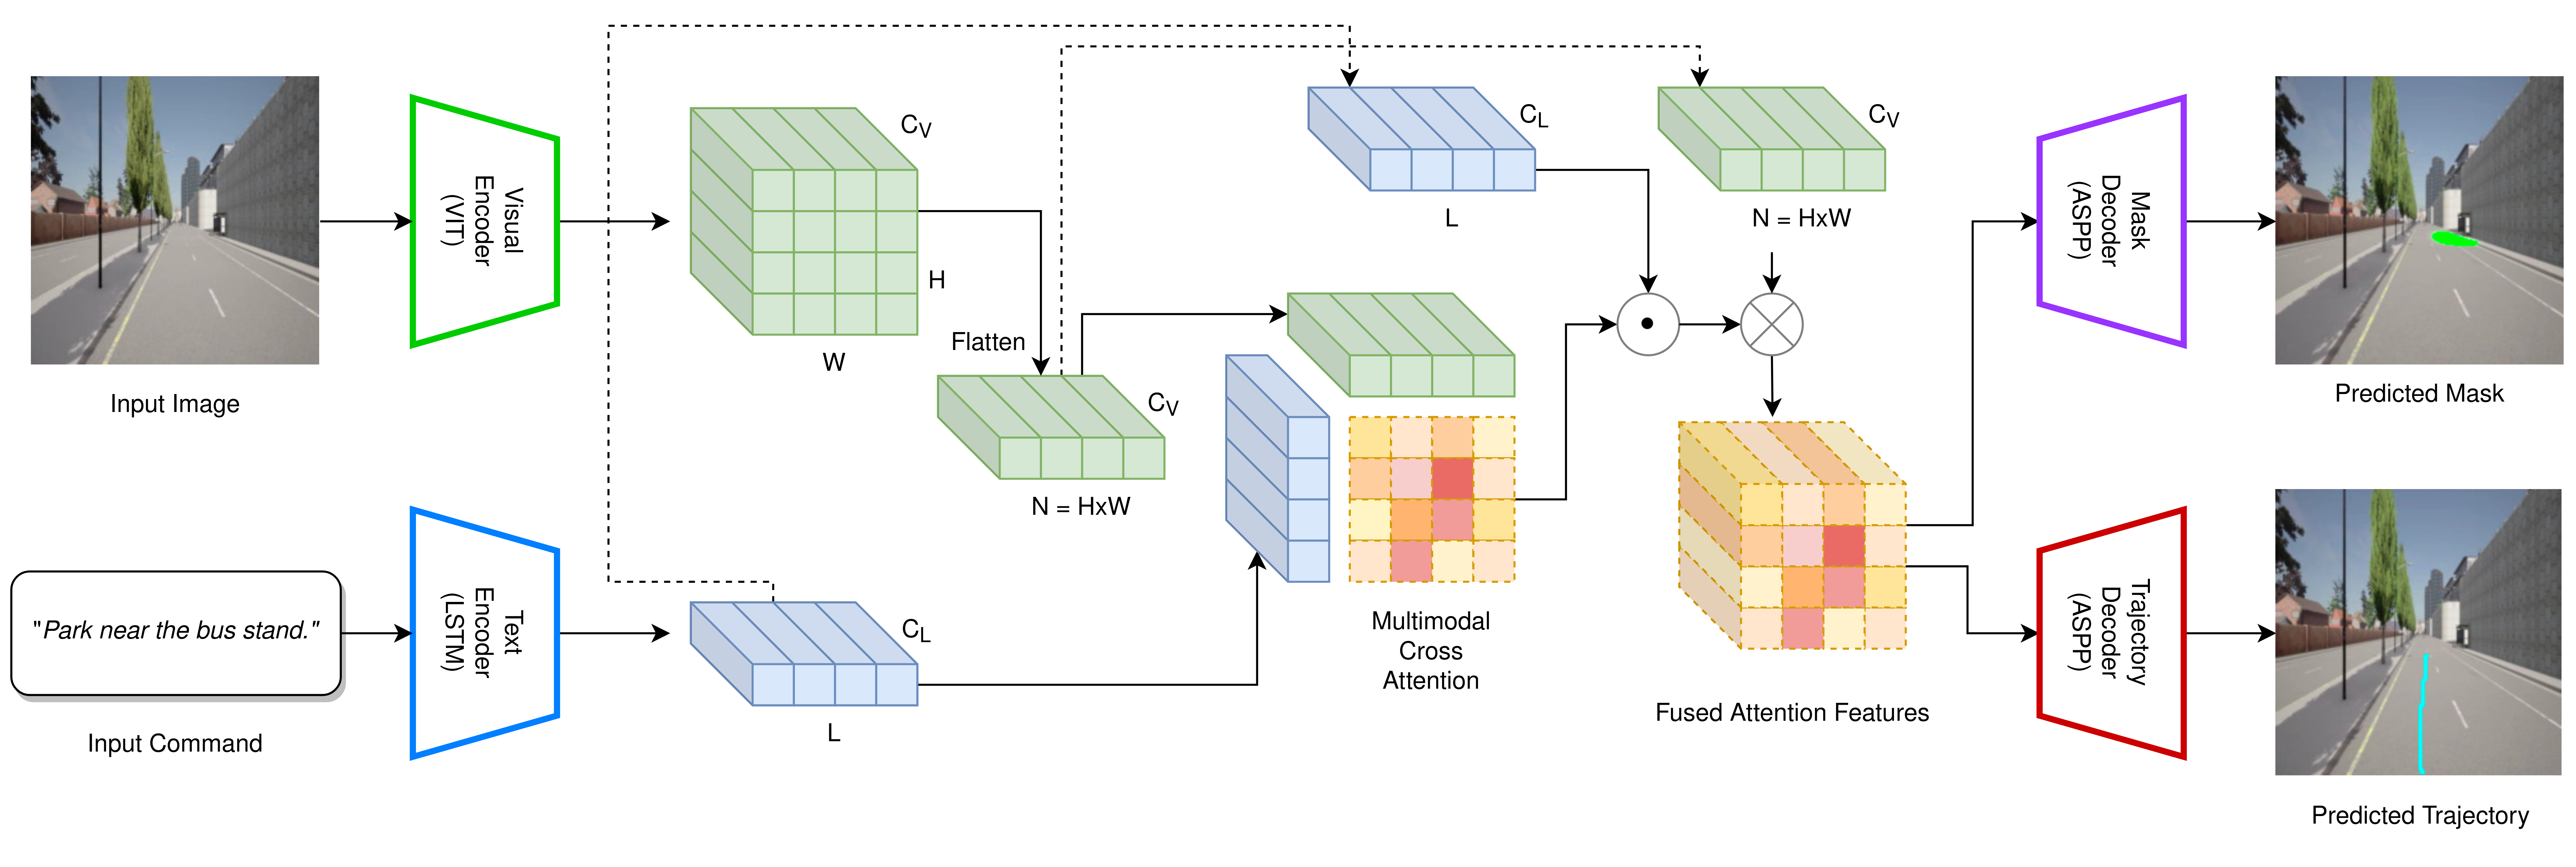
\includegraphics[width=0.95\textwidth]{figures/vln/Baseline_Model.png}
\caption[Per-frame ViT baseline]{Per-frame ViT baseline that the CLIP migration replaced: ImageNet Vision Transformer, GloVe+LSTM language stack, multimodal attention, and dual ASPP heads. The encoders are pretrained separately, so alignment must be learned entirely inside the fusion block on CARLA-NAV.}
\label{fig:vit_baseline}
\end{figure}

\subsubsection{Conv3D (X3D) Model (Multi-Frame)}

The multi-frame predecessor (Figure~\ref{fig:conv3d_model}) uses an X3D backbone~\cite{feichtenhofer2020x3d} pretrained on Kinetics-400~\cite{kay2017kinetics}. From $T=40$ input frames it samples $T=4$ frames at stride 10, extracts $C\times T\times H\times W$ features, and applies multimodal self-attention over concatenated visual and linguistic tokens (still GloVe+LSTM). A temporal convolution collapses the time axis before dual ASPP heads. Relative to the IROS draft, Conv3D upgrades fusion from pure cross-modal attention to \emph{joint} self-attention over the multimodal sequence, and introduces multi-frame visual context.

\begin{figure*}[ht]
\centering
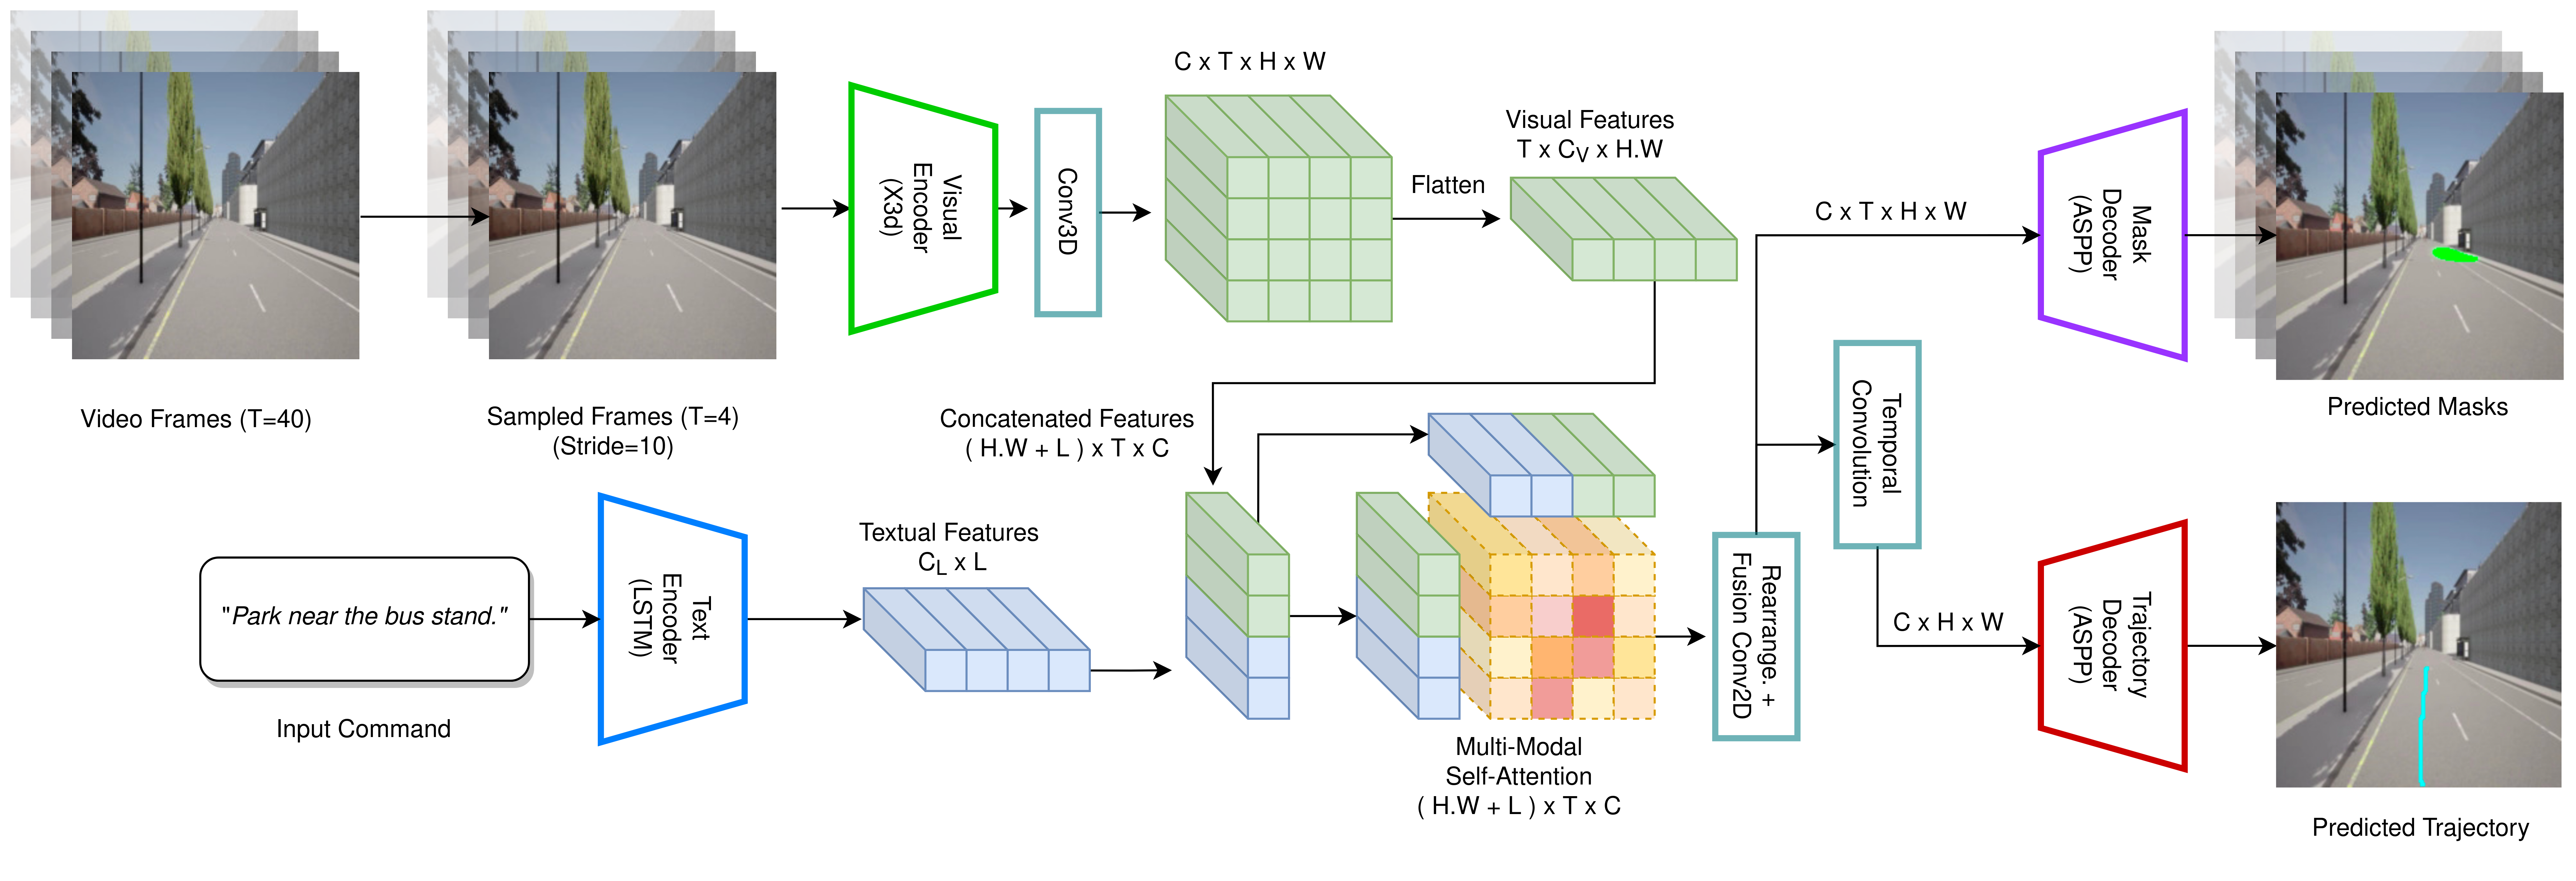
\includegraphics[width=0.98\textwidth]{figures/vln/Conv3D_Model.png}
\caption[Multi-frame Conv3D (X3D) model]{Multi-frame Conv3D (X3D) predecessor: sampled video frames through X3D, joint multimodal self-attention with LSTM language features, temporal convolution, and dual ASPP heads. Like the ViT baseline, it lacks a jointly pretrained vision--language embedding space.}
\label{fig:conv3d_model}
\end{figure*}

\subsubsection{Why CLIP}

Three considerations motivated the migration from the ViT/Conv3D lineage to CLIP. First, the GloVe+LSTM language stack has no visual grounding: word vectors are trained on text alone, so alignment with image regions must be learned entirely inside the fusion block on CARLA-NAV. CLIP~\cite{radford2021learning} instead provides a jointly pretrained image--text embedding space in which matched pairs already lie close together, giving the fusion module a stronger starting point for grounding (Section~\ref{sec:research_gaps}). Second, CARLA-NAV is small, on the order of 500 training episodes, so freezing (or lightly adapting) a large pretrained multimodal encoder is a better inductive bias than training fusion from scratch on unimodal GloVe features. Third, CLIP collapses the architecture: one dual encoder replaces the separate X3D/ViT visual backbone and LSTM language stack, simplifying training and ensuring that both modalities live in the same feature dimension ($C_v=C_l=512$). Empirically, CLIP-MC is the published outcome of that migration (Tables~\ref{table:task_completion}--\ref{table:frame_ablation}). The ViT/Conv3D numbers below document the prior art within this project; they use a different evaluation pool and metric suite, so we make \emph{no} cross-family numeric comparison.

Table~\ref{table:conv3d_vit} compares Conv3D and ViT on Fr\'{e}chet Distance, FDE, ADE, and ADE-Match (mean / median / STD; meters). Conv3D is consistently better. Critically, the standard deviation often exceeds the mean (e.g., Conv3D Fr\'{e}chet mean $17.84$ with STD $21.49$; median $9.10$), and ViT is even more heavy-tailed (mean $43.95$, STD $60.56$, median $12.19$). Path-metric means are therefore dominated by a minority of catastrophic episodes. Two further observations support the construct-validity critique in Section~\ref{sec:metric_validity}: (i)~Conv3D Fr\'{e}chet Distance and FDE nearly coincide (means $17.84$ vs.\ $17.83$; identical medians $9.10$), so the Fr\'{e}chet supremum is attained at the endpoint; the modal failure is right-path/wrong-endpoint, which ADE ($10.32$) dilutes and ADE-Match ($4.73$) hides; (ii)~over the same episodes, FDE median $9.10\,\mathrm{m}$ and ADE-Match median $1.26\,\mathrm{m}$ cannot both be faithful summaries of median quality, underscoring internal inconsistency of the displacement suite.

\begin{table}[ht]
\begin{center}
\small
\begin{tabular}{|l|ccc|ccc|}
\hline
\multirow{2}{*}{Metric} & \multicolumn{3}{c|}{Conv3D} & \multicolumn{3}{c|}{ViT} \\ \cline{2-7}
 & Mean & Median & STD & Mean & Median & STD \\ \hline
Fr\'{e}chet & 17.84 & 9.10 & 21.49 & 43.95 & 12.19 & 60.56 \\
FDE & 17.83 & 9.10 & 21.50 & 39.88 & 12.19 & 51.38 \\
ADE & 10.32 & 6.61 & 11.04 & 22.50 & 7.50 & 34.00 \\
ADE-Match & 4.73 & 1.26 & 8.51 & 16.43 & 2.50 & 31.23 \\ \hline
\end{tabular}
\end{center}
\caption{Preliminary live-navigation results for Conv3D (X3D) vs.\ ViT on the earlier evaluation pool. All values are CARLA world-frame meters. ADE values follow the regenerated evaluation tables. Lower is better for all metrics.}
\label{table:conv3d_vit}
\end{table}

\subsubsection{Stratified Ablations}

Tables~\ref{table:cmd_type}--\ref{table:subcommand} break the same evaluation down by command type, primary action verb, referred target type, and subcommand count (meters). Across strata, Conv3D remains stronger and more stable than ViT. Two qualitative patterns emerge: (i)~stopping-based commands are harder than turning-based ones for ViT (Fr\'{e}chet mean $53.98$ vs.\ $36.42$), while Conv3D is comparatively flat across both; (ii)~two-subcommand episodes yield lower Conv3D errors than single-subcommand ones (ADE $6.43$ vs.\ $12.13$), consistent with intermediate clicks providing denser supervision. These stratified tables satisfy, for the ViT/Conv3D lineage, the per-maneuver breakdown that remains open for the CLIP family (Section~\ref{sec:extended_eval}). Cross-stratum comparisons should nevertheless be read cautiously: success predicates differ by command class, endpoint-based for park/stop, state-based for lane change, sequence-based for multi-step, so a single displacement metric does not denote the same notion of difficulty in every row, and Fr\'{e}chet~$\approx$~FDE again holds in the turning stratum (both $17.97\,\mathrm{m}$ for Conv3D).

\begin{table}[ht]
\begin{center}
\small
\begin{tabular}{|l|l|ccc|ccc|}
\hline
\multirow{2}{*}{Type} & \multirow{2}{*}{Metric} & \multicolumn{3}{c|}{Conv3D} & \multicolumn{3}{c|}{ViT} \\ \cline{3-8}
 & & Mean & Med. & STD & Mean & Med. & STD \\ \hline
\multirow{4}{*}{Stopping} & ADE & 10.67 & 7.50 & 11.98 & 27.48 & 7.57 & 40.54 \\
 & ADE-Match & 4.44 & 1.37 & 9.00 & 20.90 & 3.70 & 37.59 \\
 & FDE & 17.32 & 9.67 & 21.38 & 47.67 & 12.28 & 60.74 \\
 & Fr\'{e}chet & 17.33 & 9.67 & 21.38 & 53.98 & 12.28 & 72.80 \\ \hline
\multirow{4}{*}{Turning} & ADE & 10.18 & 5.93 & 9.33 & 17.06 & 8.97 & 21.02 \\
 & ADE-Match & 5.03 & 1.32 & 7.57 & 11.40 & 3.45 & 18.25 \\
 & FDE & 17.97 & 6.97 & 21.37 & 35.57 & 16.68 & 39.78 \\
 & Fr\'{e}chet & 17.97 & 6.97 & 21.37 & 36.42 & 16.68 & 41.00 \\ \hline
\end{tabular}
\end{center}
\caption{Conv3D vs.\ ViT stratified by command type (stopping-based vs.\ turning-based). All displacement values are CARLA world-frame meters.}
\label{table:cmd_type}
\end{table}

\begin{table}[ht]
\begin{center}
\small
\begin{tabular}{|l|l|ccc|ccc|}
\hline
\multirow{2}{*}{Action} & \multirow{2}{*}{Metric} & \multicolumn{3}{c|}{Conv3D} & \multicolumn{3}{c|}{ViT} \\ \cline{3-8}
 & & Mean & Med. & STD & Mean & Med. & STD \\ \hline
\multirow{2}{*}{stop} & ADE & 11.52 & 6.83 & 13.58 & 28.15 & 8.00 & 42.68 \\
 & Fr\'{e}chet & 14.90 & 10.87 & 16.82 & 55.34 & 16.65 & 74.14 \\ \hline
\multirow{2}{*}{go} & ADE & 8.63 & 4.90 & 9.27 & 31.52 & 4.84 & 54.59 \\
 & Fr\'{e}chet & 13.72 & 8.67 & 16.60 & 52.74 & 11.07 & 86.86 \\ \hline
\multirow{2}{*}{take} & ADE & 8.99 & 4.60 & 9.22 & 19.64 & 6.36 & 23.42 \\
 & Fr\'{e}chet & 12.81 & 5.77 & 18.17 & 45.52 & 9.60 & 54.31 \\ \hline
\multirow{2}{*}{turn} & ADE & 9.17 & 4.75 & 9.23 & 17.94 & 8.03 & 22.67 \\
 & Fr\'{e}chet & 15.79 & 6.13 & 20.79 & 35.70 & 11.28 & 42.20 \\ \hline
\multirow{2}{*}{change} & ADE & 9.23 & 4.10 & 11.11 & 10.67 & 12.16 & 5.49 \\
 & Fr\'{e}chet & 21.45 & 9.67 & 26.08 & 36.76 & 33.61 & 29.80 \\ \hline
\multirow{2}{*}{drive} & ADE & 10.18 & 4.90 & 10.70 & 19.48 & 4.91 & 32.91 \\
 & Fr\'{e}chet & 15.66 & 9.92 & 19.57 & 27.60 & 9.86 & 42.71 \\ \hline
\multirow{2}{*}{park} & ADE & 6.21 & 5.32 & 5.82 & 14.43 & 4.56 & 18.97 \\
 & Fr\'{e}chet & 18.49 & 7.03 & 28.67 & 41.97 & 8.42 & 73.67 \\ \hline
\end{tabular}
\end{center}
\caption{Conv3D vs.\ ViT stratified by primary action verb (ADE and Fr\'{e}chet; meters). Full FDE/ADE-Match tables follow the same ranking and are omitted for space.}
\label{table:action_type}
\end{table}

\begin{table}[ht]
\begin{center}
\small
\begin{tabular}{|l|l|ccc|ccc|}
\hline
\multirow{2}{*}{Target} & \multirow{2}{*}{Metric} & \multicolumn{3}{c|}{Conv3D} & \multicolumn{3}{c|}{ViT} \\ \cline{3-8}
 & & Mean & Med. & STD & Mean & Med. & STD \\ \hline
\multirow{4}{*}{infrastructure} & ADE & 11.62 & 7.29 & 14.30 & 32.78 & 6.54 & 46.15 \\
 & ADE-Match & 4.84 & 1.13 & 10.66 & 26.85 & 3.02 & 44.47 \\
 & FDE & 16.79 & 9.44 & 19.27 & 55.21 & 12.04 & 70.36 \\
 & Fr\'{e}chet & 16.81 & 9.44 & 19.26 & 64.85 & 12.04 & 85.24 \\ \hline
\multirow{4}{*}{road/light} & ADE & 8.86 & 4.60 & 9.15 & 20.13 & 6.36 & 32.04 \\
 & ADE-Match & 4.21 & 1.07 & 6.94 & 14.29 & 1.72 & 29.59 \\
 & FDE & 15.64 & 7.52 & 19.48 & 33.31 & 12.69 & 37.97 \\
 & Fr\'{e}chet & 15.64 & 7.52 & 19.48 & 38.85 & 12.69 & 53.44 \\ \hline
\multirow{4}{*}{automobile} & ADE & 10.58 & 8.32 & 4.97 & 19.24 & 8.51 & 21.30 \\
 & ADE-Match & 4.15 & 2.16 & 5.29 & 14.06 & 4.61 & 20.67 \\
 & FDE & 25.48 & 13.31 & 34.69 & 47.48 & 22.17 & 45.58 \\
 & Fr\'{e}chet & 25.48 & 13.31 & 34.69 & 47.48 & 22.17 & 45.58 \\ \hline
\end{tabular}
\end{center}
\caption{Conv3D vs.\ ViT stratified by referred target type. All displacement values are CARLA world-frame meters.}
\label{table:target_type}
\end{table}

\begin{table}[ht]
\begin{center}
\small
\begin{tabular}{|c|l|ccc|ccc|}
\hline
\multirow{2}{*}{\# Subs} & \multirow{2}{*}{Metric} & \multicolumn{3}{c|}{Conv3D} & \multicolumn{3}{c|}{ViT} \\ \cline{3-8}
 & & Mean & Med. & STD & Mean & Med. & STD \\ \hline
\multirow{4}{*}{1} & ADE & 12.13 & 7.22 & 12.93 & 23.26 & 8.00 & 30.82 \\
 & ADE-Match & 6.05 & 1.29 & 9.95 & 17.30 & 3.82 & 28.93 \\
 & FDE & 21.69 & 10.58 & 24.58 & 44.78 & 13.15 & 55.70 \\
 & Fr\'{e}chet & 21.70 & 10.58 & 24.57 & 46.32 & 13.15 & 58.77 \\ \hline
\multirow{4}{*}{2} & ADE & 6.43 & 4.66 & 5.13 & 19.64 & 4.74 & 38.49 \\
 & ADE-Match & 1.91 & 1.19 & 2.49 & 14.60 & 1.26 & 36.61 \\
 & FDE & 9.64 & 7.50 & 8.65 & 29.45 & 9.11 & 40.34 \\
 & Fr\'{e}chet & 9.64 & 7.50 & 8.65 & 38.91 & 9.11 & 65.90 \\ \hline
\end{tabular}
\end{center}
\caption{Conv3D vs.\ ViT stratified by number of subcommands. All displacement values are CARLA world-frame meters.}
\label{table:subcommand}
\end{table}

\subsection{Qualitative Results}

Figure~\ref{fig:qualitative_1} compares CLIP-MC with RNR-S during live inference. Paths are overlaid on the aerial map of the CARLA environment. With multi-frame and historical trajectory context, CLIP-MC successfully performs turning and stopping maneuvers where the static-image RNR baseline fails. For ``change to the left lane,'' RNR-S continues straight while CLIP-MC changes lane (with a slight delay). In a curved-road case near a traffic light, both methods stop early, mistaking the curve for an intersection, an instructive failure mode.

\begin{figure}[ht]
\centering
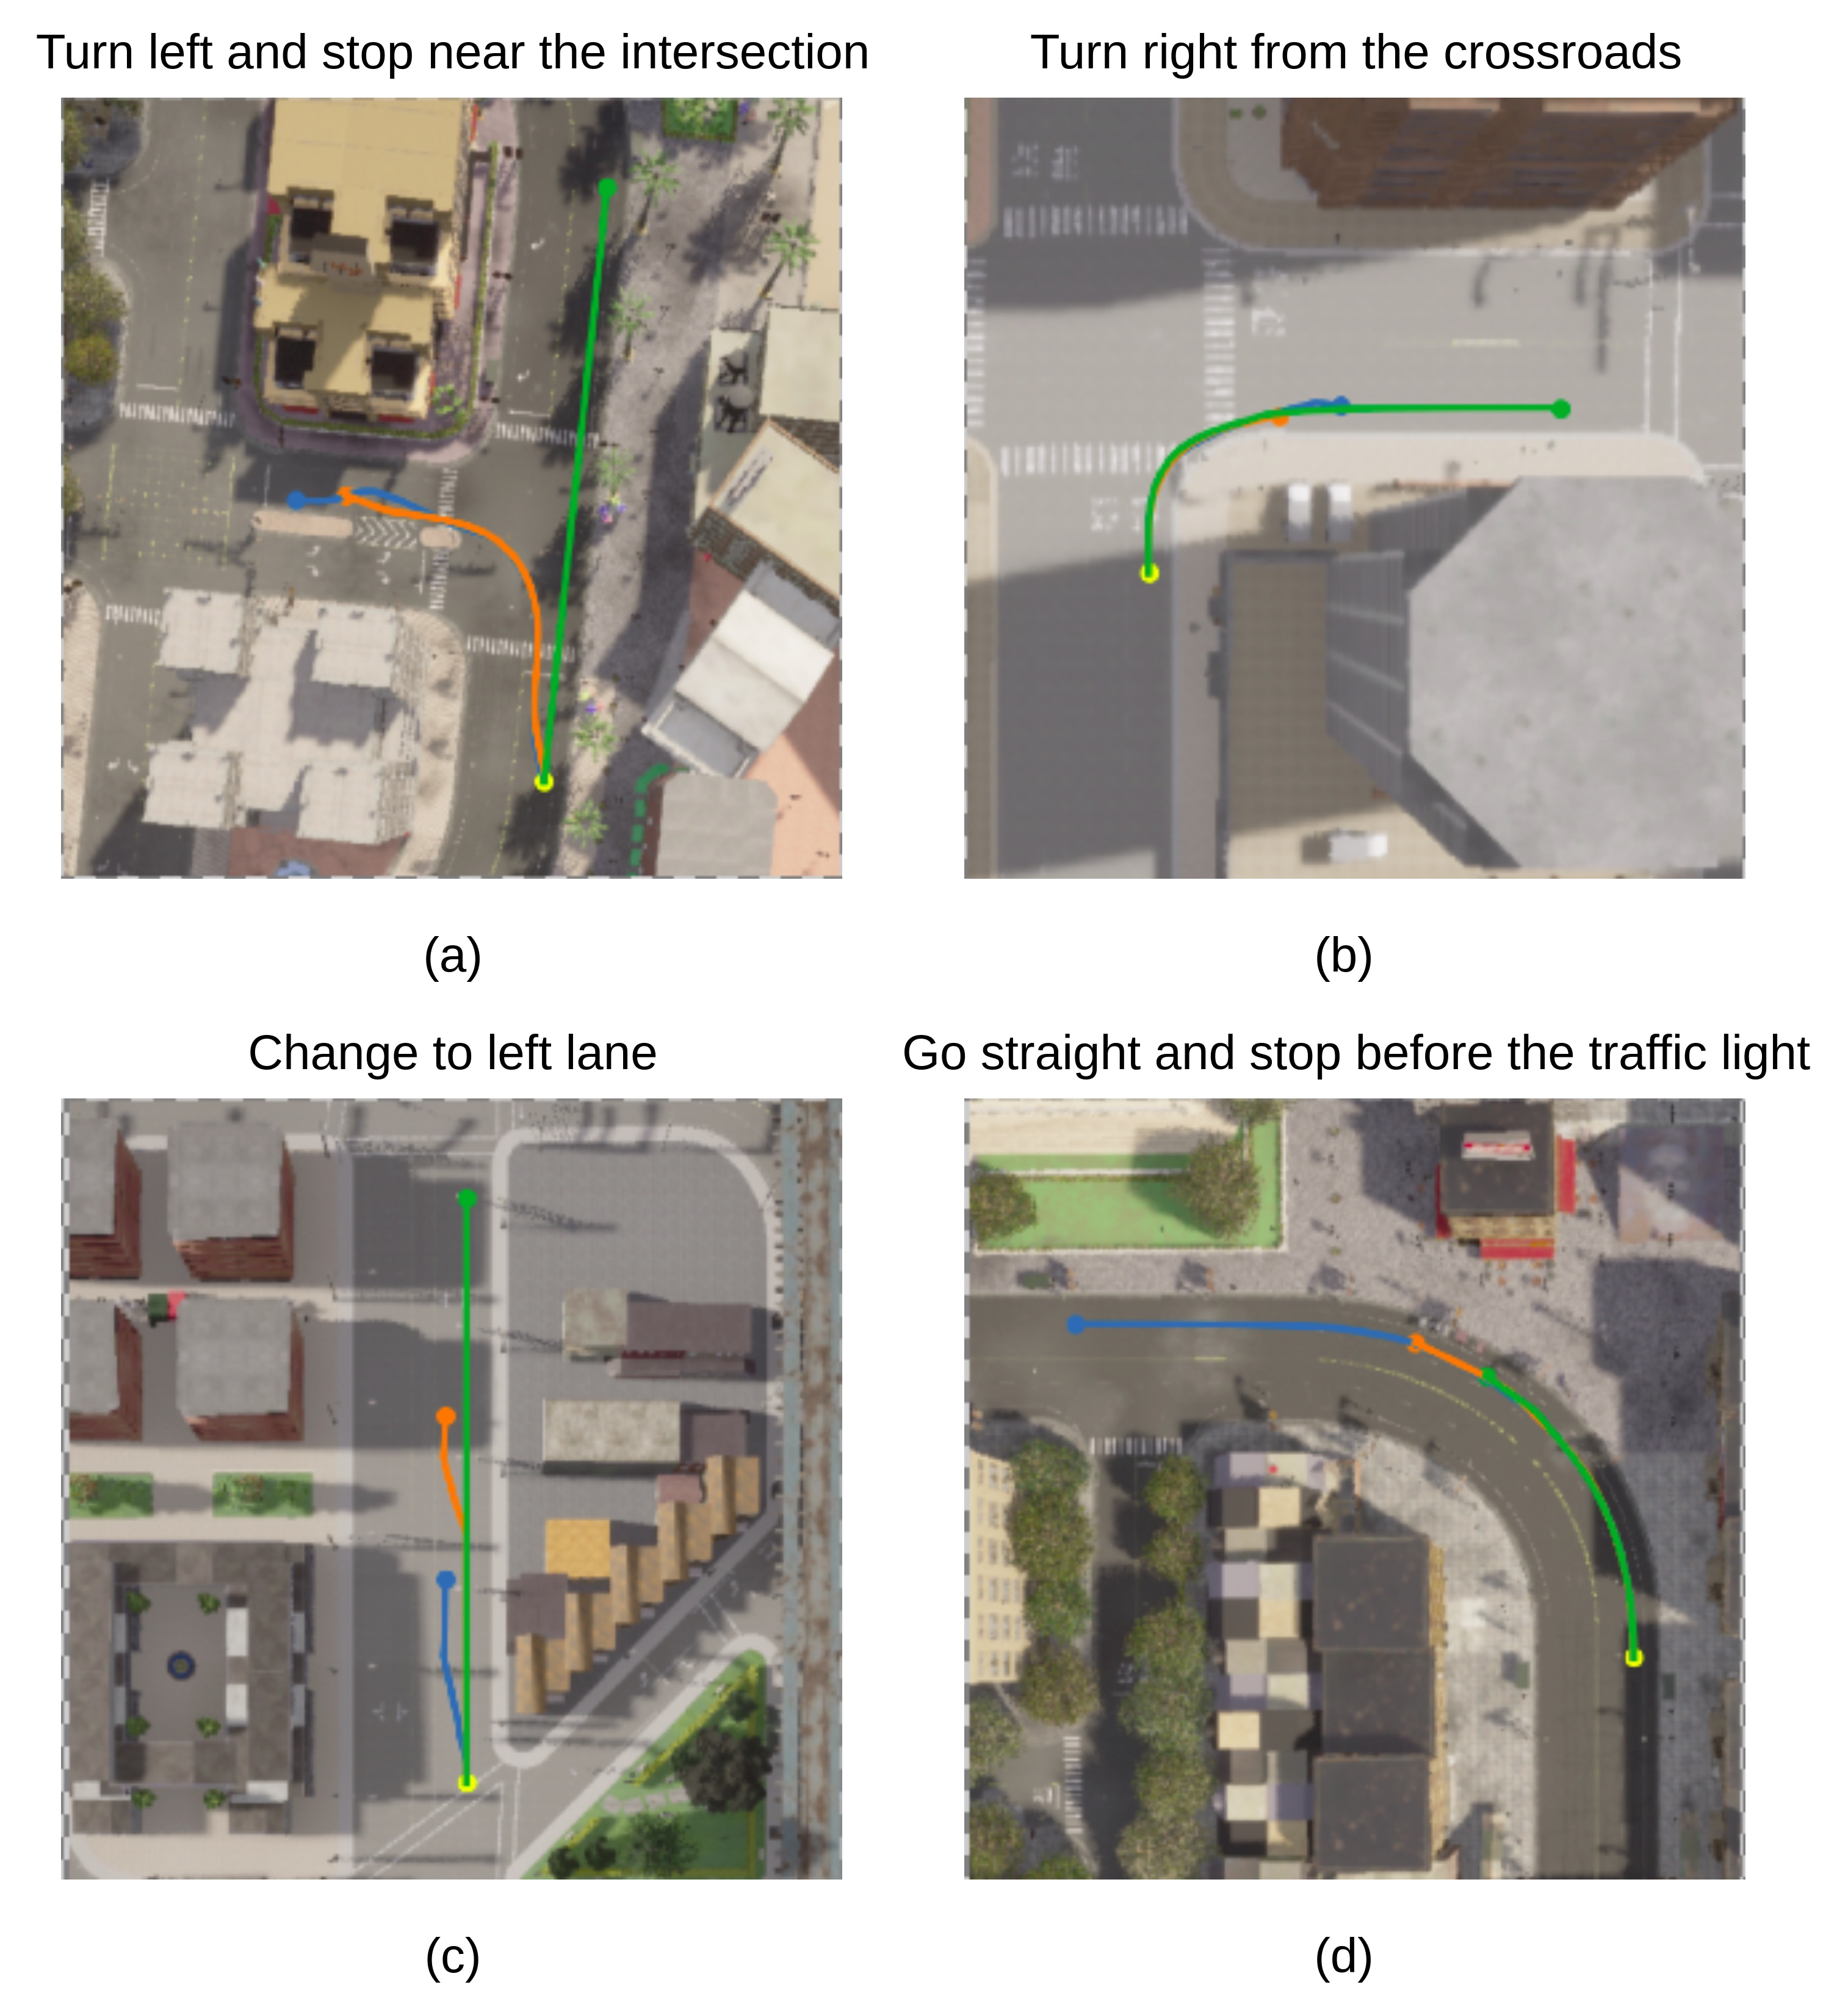
\includegraphics[width=0.55\textwidth]{figures/vln/qualitative_results_v4.jpg}
\caption[Qualitative live navigation on CARLA-NAV]{Qualitative live navigation on CARLA-NAV (yellow~=~start, orange~=~CLIP-MC, green~=~RNR-S, blue~=~ground truth). The lane-change case shows temporal context changing behavior; the curved-road case near a traffic light shows where both methods still fail by mistaking the curve for an intersection.}
\label{fig:qualitative_1}
\end{figure}

\section{Failure Modes}

Numbers alone do not reveal how the agent fails; the cases below catalog recurring live-episode patterns. Qualitative inspection of live episodes, including the cases shown in Figure~\ref{fig:qualitative_1}, reveals recurring failure patterns. Figure~\ref{fig:traj_success_fail} contrasts a successful live trajectory with a failure in which the predicted path overshoots the turn and ends far from the demonstration.

\begin{figure}[ht]
\centering
\begin{subfigure}{0.48\textwidth}
\centering
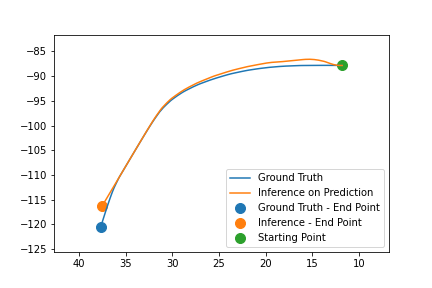
\includegraphics[width=\textwidth]{figures/vln/success_traj_1.png}
\caption{Successful trajectory alignment.}
\end{subfigure}
\hfill
\begin{subfigure}{0.48\textwidth}
\centering
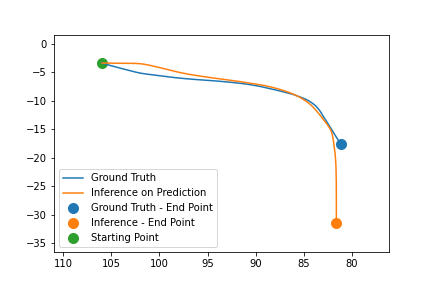
\includegraphics[width=\textwidth]{figures/vln/failure_traj_1.png}
\caption{Failure: overshot turn.}
\end{subfigure}
\caption[Success vs.\ right-path/wrong-endpoint failure]{Bird's-eye comparison of ground-truth (blue) and live inferred (orange) trajectories (green~=~start; colored dots mark endpoints). The failure is right-path/wrong-endpoint: the same pattern that Fr\'{e}chet~$\approx$~FDE quantifies in Table~\ref{table:conv3d_vit} and that motivates Task Completion as the primary metric.}
\label{fig:traj_success_fail}
\end{figure}

\begin{enumerate}
    \item \textbf{Delayed lane change:} On commands such as ``change to the left lane,'' CLIP-MC eventually executes the maneuver but with a slight delay relative to the ground-truth path, while RNR-S may continue straight. Temporal context helps, but reaction lag remains.
    \item \textbf{Curve mistaken for an intersection:} On a curved road approaching a traffic light, both CLIP-MC and RNR-S stop prematurely, treating the geometry as an intersection. This suggests sensitivity to road layout cues that resemble junction structure.
    \item \textbf{Early stopping from the area threshold:} When several candidate goal regions are visible, the area-based stopping rule can fire before the intended final region is reached, because a large connected component satisfies the empirical threshold for five consecutive predictions. Area growth under perspective is a proxy for proximity, not for identity of the correct region; Section~\ref{sec:discussion} returns to this point.
    \item \textbf{Referential ambiguity and path metrics:} Commands such as ``park near the blue dustbin'' admit multiple valid stopping locations. Fr\'{e}chet Distance and nDTW then penalize a spatially plausible path that differs from the recorded demonstration, even when Task Completion may still succeed.
    \item \textbf{Synthetic-to-real domain gap:} All training and evaluation are in CARLA. Appearance, sensor noise, and traffic behavior in the real world differ, so transfer without domain adaptation~\cite{kundu2021generalize,kang2020pixel} is an open risk (Section~\ref{sec:vln_limitations}).
\end{enumerate}

\section{Discussion}
\label{sec:discussion}

The tables above establish what happens; this section asks why, why it is interesting, and why it is useful. Failure patterns themselves are catalogued in the previous section and are not repeated here.

\paragraph{Trajectory context helps most with multiple frames.}
Historical contextual trajectory improves validation TC by one episode for single-frame models (CLIP-SC $0.52$ vs.\ CLIP-S $0.48$) but by four episodes once multi-frame visual input is present (CLIP-MC $0.72$ vs.\ CLIP-M $0.56$). Why? A single frame has no way to distinguish ``before the turn'' from ``after the turn,'' so the past-trajectory map is the only progress signal available; with eight frames the model can also read motion, and the two turn out to be complementary rather than redundant. This is interesting because it tracks instruction progress without an explicit instruction-segmentation module. It is useful because it suggests that progress context and short-term visual history should be designed as a pair, not as interchangeable substitutes.

\paragraph{Fr\'{e}chet Distance $\approx$ FDE is a diagnosis, not a coincidence.}
For Conv3D, Fr\'{e}chet Distance and FDE means nearly coincide ($17.84$ vs.\ $17.83\,\mathrm{m}$) with identical medians ($9.10$). The supremum is attained at the terminal point in essentially every episode, so the modal failure is right-path/wrong-endpoint. That is interesting because it tells a follow-up to spend effort on the stopping rule rather than on path following. It is also the direct empirical justification for the geometric goal-region predicate in Section~\ref{sec:reproducible_tc}: if the path is usually fine and the endpoint is the problem, a predicate on the final pose is the right primary metric.

\paragraph{Why RNR-SC can win on validation path metrics yet lose on test TC.}
On validation, RNR-SC outperforms CLIP-S, CLIP-SC, and CLIP-M on Fr\'{e}chet Distance and nDTW, even though CLIP variants are stronger on test Task Completion. Two competing hypotheses remain open. First, sup-driven metrics on 25 episodes can be dominated by one catastrophic outlier, so a backbone that avoids a single bad episode looks stronger without being so on average. Second, CLIP may ground better across maps (hence higher test TC) while driving less smoothly on the small validation pool (hence worse path metrics). The first hypothesis is testable by reporting medians and bootstrap CIs; the second requires a map-unseen protocol (Section~\ref{sec:extended_eval}). We do not assert either; the discrepancy is itself a reason not to over-interpret intermediate path-metric rankings.

\paragraph{Two-subcommand episodes score better than single-subcommand ones.}
Conv3D ADE is $6.43\,\mathrm{m}$ on two-subcommand episodes versus $12.13\,\mathrm{m}$ on single-subcommand ones. The denser-supervision explanation (intermediate clicks supply more mask targets) is plausible, but it is confounded with episode length and command difficulty. A length-controlled check would be needed before treating this as a design recommendation.

\paragraph{Path-metric dispersion sets a noise floor on Table~\ref{table:path_metrics}.}
Standard deviations often exceed the means in Table~\ref{table:conv3d_vit}. Gaps of a few units among non-CLIP-MC rows in Table~\ref{table:path_metrics} therefore sit inside episode-level dispersion. Aggregate path metrics remain useful for spotting the CLIP-MC jump; they are a poor basis for ranking the intermediate rows.

\paragraph{Area-threshold stopping fires on size, not identity.}
As noted under Failure Modes, the area rule can stop early when several candidate regions are visible. Area growth under perspective proxies proximity, not identity of the referred region. Future stopping rules should therefore combine area with semantic confirmation of referred objects or confidence-aware temporal consistency~\cite{xiang-etal-2020-learning}.

\paragraph{Set-valued targets unify the metric and the head.}
The same observation that a command designates a \emph{set} $\Phi(C)$ of valid trajectories (Section~\ref{sec:metric_validity}) explains both why Task Completion is the primary metric and why the output head is a segmentation map rather than a coordinate regressor. A regressor trained under squared loss converges to the conditional mean of the valid modes; for ``park between the two cars,'' that mean sits in the middle of the road and is not itself a valid goal. A segmentation head places mass on multiple disjoint valid regions and recovers a mode via the largest connected component. The thesis previously applied this insight only to evaluation; stating it here connects the metric argument to the architectural one.

\section{Limitations}
\label{sec:vln_limitations}

The discussion above already flags stopping-rule and metric issues; three broader limitations constrain real-world claims. A major limitation that restricts real-world practicality is the synthetic nature of CARLA-NAV; domain adaptation~\cite{kundu2021generalize,kang2020pixel} is required before claiming transfer to real imagery. The stopping criterion is rule-based rather than learned; learning when to stop~\cite{xiang-etal-2020-learning} is more scalable (see Failure Modes and Discussion). Finally, the predicted future trajectory currently serves interpretability only; incorporating it into the planner for end-to-end navigation remains future work. These limitations were drafted for an earlier conference submission and omitted from the archival six-page version for space; we restore them here for thesis-level completeness.

\section{Extended Evaluation Protocol}
\label{sec:extended_eval}

The ICRA evaluation protocol underlying Tables~\ref{table:task_completion}--\ref{table:frame_ablation} is limited in several ways that matter for a thesis-level claim. We document those limits, report what can be derived without re-training (Wilson CIs above; ViT/Conv3D stratified tables), and specify the protocols we adopt for stronger evaluation. Where new live runs were not available for this manuscript, we state the intended measurement explicitly rather than implying the current tables already cover it.

\subsection{Held-Out Map Split}

The default CARLA-NAV splits shuffle episodes across eight maps, so train, validation, and test can share map layouts (Chapter~\ref{ch:dataset}). Following the seen/unseen convention of R2R~\cite{anderson2018vision}, we define a \textbf{map-unseen} protocol: train on six maps, validate on one held-out map, and test on the remaining map (rotated so each map appears in test across folds). Under this protocol, Task Completion, Fr\'{e}chet Distance, and nDTW should be reported separately for map-seen and map-unseen episodes. The numbers in Tables~\ref{table:task_completion}--\ref{table:frame_ablation} use the original shuffled split and therefore do \emph{not} establish cross-map generalization; they are an upper bound relative to a true unseen-map evaluation.

\subsection{Multi-Seed Confidence and Stochastic Live Traffic}

Live CARLA episodes are stochastic under dynamic traffic. A single evaluation pass yields the point estimates above; Table~\ref{table:tc_ci} adds Wilson intervals for that pass, but does not capture seed-to-seed variance of training or of traffic randomization, nor human-annotator disagreement on TC (see Section~\ref{sec:eval_metrics} for the same caveat). The recommended protocol is: train with at least three random seeds, evaluate each checkpoint on the live val/test suites with fixed spawn poses but resampled traffic, and report mean $\pm$ standard deviation of TC together with bootstrap CIs for path metrics. Overlapping Wilson intervals for CLIP-MC vs.\ CLIP-M on validation already caution against overstating single-run deltas.

\subsection{Safety and Infractions}

Task Completion records goal arrival but not \emph{how} the vehicle drove. We therefore include CARLA's built-in sensors in the evaluation contract:

\begin{itemize}
    \item \textbf{Collisions:} count of collision events (vehicles, pedestrians, static props) per episode and per kilometer.
    \item \textbf{Lane invasions:} cumulative lane-invasion sensor triggers.
    \item \textbf{Traffic-light infractions:} red-light violations recorded by the simulator's traffic-light API.
\end{itemize}

An episode may count as Task Completion success yet still be unacceptable under these rates. Infractions were not logged in the original ICRA runs; subsequent live evaluation should report them alongside TC.

\subsection{Reproducible Goal-Region Success Predicate}
\label{sec:reproducible_tc}

Human TC relocates the construct problem into the annotator (Section~\ref{sec:metric_validity}). CARLA-NAV already stores annotated final and intermediate navigable regions, so success can be redefined as a reproducible geometric predicate that still admits multiple valid paths:

\begin{enumerate}
    \item \textbf{Goal arrival:} the final vehicle pose lies within radius $r$ of the annotated final navigable region (equivalently, within the region or its $r$-dilation in world coordinates).
    \item \textbf{Subcommand constraints:} for multi-step commands, the trajectory visits each annotated intermediate navigable region (again up to radius $r$) in order.
    \item \textbf{Legality:} the episode incurs zero collisions and zero red-light infractions under the CARLA sensors listed above; lane invasions may be reported separately rather than hard-failed, depending on the maneuver class.
\end{enumerate}

An episode succeeds only if all three hold. The radius $r$ should be chosen on a held-out calibration set and reported; a natural default is on the order of the final-region diameter used during annotation. This predicate answers both halves of the right-path/wrong-endpoint dichotomy: the endpoint is checked against the annotated goal set rather than a single demonstration pose, and intermediate regions encode the path constraints that FDE alone misses.

\paragraph{Calibration experiments.}
Two measurements are needed before displacement scores or geometric TC can be interpreted absolutely: (i)~an \emph{annotation noise floor}, re-collect a subset of episodes with a second navigator and report ADE/FDE between the two human trajectories under matched traffic seeds, estimating click-placement variance; (ii)~a \emph{traffic stochasticity floor}, roll out a fixed checkpoint repeatedly from the same spawn with resampled traffic and report the dispersion of path metrics and geometric TC. Neither was measured in the ICRA runs; both belong in any follow-up that claims absolute navigation quality.

\subsection{Trajectory-Head Ablation, Per-Maneuver Breakdown, and Runtime}

\begin{itemize}
    \item \textbf{Trajectory head:} Train a navigation-only variant (CLIP-MC without the $z_t$ head) and compare TC and path metrics to the full multi-task model. Separately score the trajectory head with soft Dice / IoU against projected ground-truth short-horizon paths. Without this ablation, Contribution~\ref{contrib:network} rests on interpretability alone (as noted in Section~\ref{sec:contributions}).
    \item \textbf{Per-maneuver breakdown:} For the ViT/Conv3D lineage, Tables~\ref{table:cmd_type}--\ref{table:subcommand} already provide stratified displacement metrics by command type, action verb, target type, and subcommand count. The corresponding TC-stratified breakdown for the CLIP family (turn, straight, stop, park, multi-step) remains future work; aggregate CLIP metrics can still hide systematic failure on parking or lane-change commands.
    \item \textbf{Runtime:} Profile wall-clock milliseconds per forward pass (CLIP encode + fusion + heads) and end-to-end control frequency (Hz) on the live inference machine, with and without the every-5-frame schedule. The complexity argument in Section~\ref{sec:formal_analysis} predicts quadratic growth in $T$; measured latency makes that claim concrete.
\end{itemize}

\subsection{Ethics and Deployment Safety}

Language-guided driving systems can fail silently under referential ambiguity, domain shift, or planner error. We do not claim readiness for real vehicles: all results are in simulation, collision metrics are not yet reported, and synthetic-to-real transfer remains open. Any deployment path would require redundant safety layers (collision checking, human override, and conservative stopping) independent of the grounding network.

\section{Chapter Summary}

We reformulated RNR for dynamic outdoor VLN, motivated the grounding-first design formally, introduced a multi-task network with CLIP features, multi-frame context, and historical trajectory, and demonstrated live navigation in CARLA. We also documented the preliminary ViT and Conv3D architectures and their stratified displacement results, and argued that Task Completion, not ADE/FDE/ADE-Match, is the appropriate primary metric because language commands specify sets of valid trajectories rather than a single demonstration path. Quantitative CLIP results show that CLIP-MC outperforms single-frame and non-contextual baselines on Task Completion, Fr\'{e}chet Distance, and nDTW, with Wilson intervals, human-TC disclosure, path-metric dispersion caveats, and the extended evaluation protocol clarifying the statistical and safety limits of those gains. The next chapter concludes the thesis and outlines future work.
